\documentclass[11pt]{article}
\usepackage[margin=1in]{geometry}
\usepackage{amsmath,amssymb}
\usepackage{booktabs}
\usepackage{graphicx}
\usepackage{xcolor}
\usepackage{hyperref}
\usepackage{tikz}
\usetikzlibrary{positioning,arrows.meta,fit,backgrounds}
\usepackage{caption}
\captionsetup{font=small}
\hypersetup{colorlinks=true,linkcolor=blue,citecolor=blue,urlcolor=blue}

\graphicspath{{figs/}}
\newcommand{\todo}[1]{\textcolor{red}{[\textsc{todo}: #1]}}
\newcommand{\approxeqq}{\ensuremath{\approx}}

\title{\textbf{Compress the Latent Relay:\\[2pt]
\large Why Multi-Agent KV Caches Shrink 16--40$\times$}\\[4pt]
\large Causal evidence that inter-agent latent communication is not an
information channel}

\author{Sagnik Biswas \\ \small (advisor: Jiayi Tian) \\[4pt]
\small Preliminary draft --- \today.}
\date{}

\begin{document}
\maketitle

\begin{abstract}
Latent multi-agent systems such as LatentMAS~\cite{latentmas} let intermediate
agents share a key--value (KV) cache instead of text, on the assumption that this
cache carries richer problem-specific reasoning to the final reader. We show that
assumption is largely false---and that the practical consequence is extreme
\textbf{cache compression}.

With a controlled intervention protocol (swap / remove / compress the relay
cache under matched decoding budgets), we find the reader is insensitive to
\emph{instance-level} content: a different same-task question's cache matches the
correct one on accuracy, the answer is barely decodable from upstream latents,
and three steering methods fail to improve accuracy through the channel. The
cache instead acts as a content-independent decoding-mode scaffold. Because
instance content does not matter, the relay is highly redundant: plain headwise
eviction compresses it \textbf{16--40$\times$} at iso-accuracy on GSM8K
($100\,$MB$\to 2.5\,$MB), and reader-side concision steering removes any
verbosity tax from aggressive compression. On harder MATH the compression is no
longer free (accuracy dips; tokens rise), giving a clear task boundary. A fixed
synthetic cache that skips upstream agents is a consistent corollary, not the
main result. The usable systems lever in latent multi-agent inference is
\textbf{compress the relay (and optimize the reader)}, not enrich the latent
channel.
\end{abstract}

% ======================================================================
\section{Introduction}
Multi-agent LLM pipelines decompose reasoning across roles (plan / critique /
refine) that exchange messages. \emph{LatentMAS}~\cite{latentmas} replaces those
text messages with a shared KV cache: upstream agents run latent forward passes,
emit no tokens, and grow \texttt{past\_key\_values} that the final agent (the
\emph{reader}) consumes before decoding. The design assumes the cache is an
\textbf{information channel} carrying problem-specific intermediate reasoning.

We test that assumption causally and get a systems answer. The reader does
\emph{not} rely on problem-specific cache content: swapping in another
same-task question's cache leaves accuracy essentially unchanged; probes cannot
read out the answer from upstream latents; and steering the latent channel
cannot raise accuracy. What remains is a weaker effect---a shared decoding mode
that often shortens the reader's chain-of-thought under tight budgets.

If instance-level content does not matter, the relay should be compressible.
We show that it is. Applying standard KV eviction (sink + top-$k$ positions per
layer) to the multi-agent relay yields \textbf{16--40$\times$} memory reduction
at matched accuracy on GSM8K; when aggressive compression makes the reader more
verbose, a reader-only steering vector removes that tax. Compression is the
headline exploit; mechanism results explain \emph{why} it is nearly free; a
synthetic (question-independent) cache that skips upstream compute is a
corollary. On harder MATH, compression begins to cost accuracy---a boundary, not
a contradiction of content-independence (wrong-question caches still match).

\paragraph{Contributions.}
\begin{enumerate}\itemsep2pt
\item A \textbf{causal intervention protocol} for latent multi-agent systems
(real / shuffled / none / compressed cache $\times$ budget, plus probes) that
separates content from presence (\S\ref{sec:protocol}).
\item Evidence that the latent relay is \textbf{not an instance-specific
information channel}: real $\approxeqq$ shuffled, weak upstream readout, and
failed accuracy steering (\S\ref{sec:steer}--\ref{sec:mechanism}).
\item A \textbf{compression exploit}: 16--40$\times$ inter-agent KV reduction at
iso-accuracy on GSM8K via plain eviction, with reader-side steering cancelling
the verbosity tax; MATH as a task boundary (\S\ref{sec:exploit}).
\end{enumerate}

% ======================================================================
\section{Background and Setup}
\label{sec:bg}
\paragraph{LatentMAS.} We use a verified, byte-for-byte reproduction of
LatentMAS~\cite{latentmas}:
\textbf{Planner\,$\to$\,Critic\,$\to$\,Refiner\,$\to$\,Judger}. Unless noted,
each upstream agent runs $K{=}40$ latent steps and appends to a shared KV cache;
only the Judger decodes (Fig.~\ref{fig:arch}). Our fork matches the paper's
reported accuracy on Qwen3-14B within a few points (GSM8K 92.7 vs.\ 95.2; ARC-C
94.7 vs.\ 95.6; MedQA 79.3 vs.\ 80.7).

\paragraph{KV compression of the relay.} After the upstream agents finish, we
compress their joint cache before the Judger reads it: keep a few sink positions
plus the top-$k$ by per-layer importance (key-norm by default), optionally with a
low-rank back-fill of evicted mass (OBF). This applies H2O/SnapKV-style
eviction~\cite{h2o,snapkv} to a \emph{multi-agent latent relay} rather than a
single long context.

\paragraph{Reader-side concision steering (ASC).} When compression makes the
reader verbose, we add a training-free SEAL residual~\cite{seal},
$v=\mathrm{mean}(\text{execution})-\mathrm{mean}(\text{reflection}\cup\text{transition})$,
to the Judger's residual stream only. Upstream agents stay unsteered.

\begin{figure}[t]
\centering
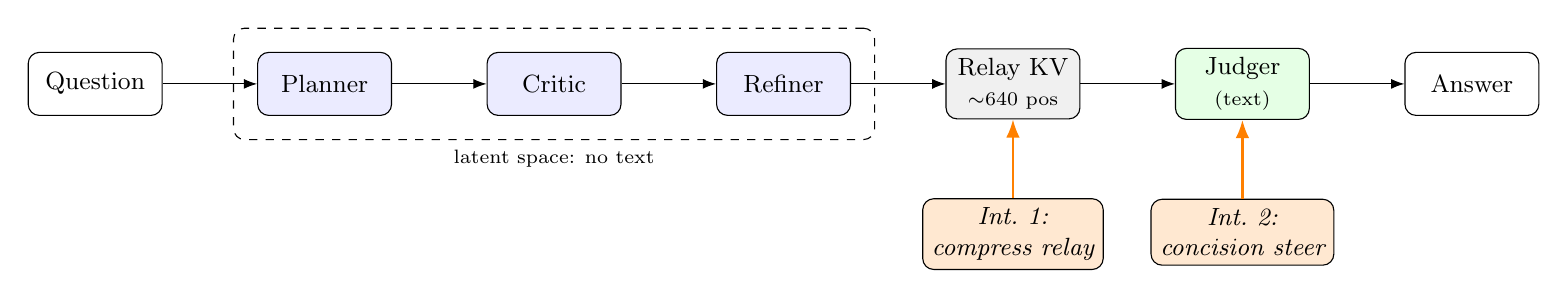
\begin{tikzpicture}[
  node distance=8mm and 12mm,
  box/.style={draw,rounded corners,minimum height=8mm,minimum width=17mm,font=\small,align=center},
  lat/.style={box,fill=blue!8},
  jud/.style={box,fill=green!10},
  interv/.style={draw,rounded corners,fill=orange!18,font=\small\itshape,align=center,minimum height=7mm},
  >=Latex]
  \node (q) [box] {Question};
  \node (p) [lat,right=of q] {Planner};
  \node (c) [lat,right=of p] {Critic};
  \node (r) [lat,right=of c] {Refiner};
  \node (kv) [box,fill=gray!12,right=of r,align=center] {Relay KV\\ \scriptsize $\sim$640 pos};
  \node (j) [jud,right=of kv] {Judger\\\scriptsize (text)};
  \node (a) [box,right=of j] {Answer};
  \draw[->] (q)--(p); \draw[->] (p)--(c); \draw[->] (c)--(r); \draw[->] (r)--(kv);
  \draw[->] (kv)--(j); \draw[->] (j)--(a);
  \begin{scope}[on background layer]
    \node[draw,dashed,rounded corners,fit=(p)(c)(r),inner sep=3mm,label=below:{\scriptsize latent space: no text}] {};
  \end{scope}
  \node (comp) [interv,below=10mm of kv] {Int.~1:\\compress relay};
  \node (asc) [interv,below=10mm of j] {Int.~2:\\concision steer};
  \draw[->,orange,thick] (comp)--(kv);
  \draw[->,orange,thick] (asc)--(j);
\end{tikzpicture}
\caption{LatentMAS and our interventions. Upstream agents grow a shared KV
relay; only the Judger emits text. \textbf{Int.~1} compresses the relay
(memory). \textbf{Int.~2} steers the reader (verbosity).}
\label{fig:arch}
\end{figure}

\paragraph{Models and tasks.} Primary: Qwen3-14B; cross-scale: Qwen3-4B.
Tasks: GSM8K (main compression suite), MedQA (mechanism), MATH-500 (harder
boundary). \todo{Llama-3.1-8B cross-family; AIME at $K{=}10$ (see
\S\ref{sec:limits}).} Greedy decode unless noted; paired bootstrap 95\% CIs.

% ======================================================================
\section{A Causal Intervention Protocol}
\label{sec:protocol}
Correlational gains from adding latent agents are ambiguous: they may transmit
reasoning, or merely shift the reader's decoding mode. We hold the Judger prompt
fixed and replace the cache it reads:
\begin{itemize}\itemsep2pt
\item \textbf{real}: item's own upstream cache.
\item \textbf{shuffled}: another same-task question's real cache (wrong content,
on-manifold).
\item \textbf{none}: no relay (Judger-only).
\item \textbf{compressed}: real cache after eviction / OBF (\S\ref{sec:exploit}).
\item \textbf{synthetic} (corollary): fixed cache sampled from population
per-channel statistics of real caches.
\end{itemize}
The decisive comparison is \textbf{real vs.\ shuffled}. We also probe upstream
latents for the gold answer and ablate upstream roles.

% ======================================================================
\section{Result 1: The Channel Is Not Steerable for Accuracy}
\label{sec:steer}
If the relay were an information channel, steering its content should help. Three
methods fail (Table~\ref{tab:steer}): training-free correctness-contrastive
residuals on upstream latents; one-shot KV hand-off steering; and an end-to-end
learned residual through a differentiable KV path (inert or destructive-only).
No method finds an accuracy-improving direction. Leverage is not inside the
latent channel.

\begin{table}[t]
\centering\small
\caption{Steering latent content does not improve accuracy (Qwen3-14B unless
noted).}
\label{tab:steer}
\begin{tabular}{@{}lll@{}}
\toprule
Method & Setting & Outcome \\
\midrule
Diff-of-means (upstream) & GSM8K/ARC/MedQA & within noise; hurts MedQA \\
KV-cache hand-off steering & GSM8K & falsified (saturates/corrupts) \\
Learned residual (diff.\ KV) & 4B/MedQA & inert or destructive-only \\
\bottomrule
\end{tabular}
\end{table}

% ======================================================================
\section{Result 2: The Channel Is Not Instance-Specific}
\label{sec:mechanism}
\paragraph{Real $\approxeqq$ shuffled.} Table~\ref{tab:swap}: a wrong-question
same-task cache matches the correct one on MedQA, GSM8K, and MATH. Removing the
cache (\textbf{none}) hurts under tight budgets on MedQA/GSM8K, but the gap
shrinks as the budget grows---much of the apparent upstream benefit is a
decoding-budget artifact.

\paragraph{Cross-task.} A MedQA donor cache on MATH matches real accuracy in our
$n{=}60$ run (Table~\ref{tab:swap}), so domain jumps are not automatically fatal;
we do not claim arbitrary cross-domain free lunch. \todo{MedQA$\leftarrow$GSM8K
donor cell for symmetry.}

\paragraph{Weak upstream readout.} Linear/MLP probes for the gold answer sit near
chance on Planner/Critic/Refiner; only the Judger shows a clear correctness
signal (Table~\ref{tab:probe}).

\begin{table}[t]
\centering\small
\caption{Content-independence. Accuracy at decoding budget $T$. Shuffled $=$
wrong-question same-task cache; crosstask donor noted in parentheses.}
\label{tab:swap}
\begin{tabular}{@{}llrrrrr@{}}
\toprule
Model & Task & $T$ & real & shuf & none & notes \\
\midrule
Qwen3-14B & MedQA & 1024 & 0.675 & 0.625 & 0.350 & \\
Qwen3-14B & MedQA & 4096 & 0.800 & 0.775 & 0.750 & gap collapses \\
Qwen3-14B & GSM8K & 1024 & 0.933 & 0.933 & 0.800 & \\
Qwen3-4B  & MedQA & 1024 & 0.450 & 0.450 & 0.150 & \\
Qwen3-14B & MATH  & 2048 & 0.783 & 0.783 & 0.700 & MedQA donor also 0.783 \\
\bottomrule
\end{tabular}
\end{table}

\begin{table}[t]
\centering\small
\caption{Upstream latents barely encode the answer (chance gold acc $0.25$).}
\label{tab:probe}
\begin{tabular}{@{}lrr@{}}
\toprule
Agent & gold acc (MLP) & correctness AUC \\
\midrule
Planner & 0.33 & 0.54 \\
Critic  & 0.32 & 0.62 \\
Refiner & 0.28 & 0.59 \\
\textbf{Judger} & --- & \textbf{0.69--0.80} \\
\bottomrule
\end{tabular}
\end{table}

% ======================================================================
\section{Result 3: Compress the Relay}
\label{sec:exploit}
Content-independence predicts redundancy. We make that operational.

\paragraph{16--40$\times$ at iso-accuracy (GSM8K).}
Table~\ref{tab:comp} and Fig.~\ref{fig:2x2}: full $2{\times}2$ on
GSM8K/Qwen3-14B (relay $\in$\{full, compressed\} $\times$ ASC
$\in$\{off, on\}). Keeping 32 positions ($16\times$ smaller KV) preserves
accuracy. At 16--24 positions ($27$--$40\times$; $100\,$MB$\to 2.5$--$3.75\,$MB),
accuracy stays within noise; \textbf{plain headwise eviction} (no OBF back-fill)
matches the full baseline at $0.817$ with the least memory.

\paragraph{Verbosity tax is separable.} Aggressive compression adds
$+37$ tokens ($95\%$ CI $[+11,+67]$). Reader-only ASC removes it
($-44$ $[-71,-16]$) and restores steered full-cache accuracy. Interaction
$\approx 0$: ASC transfers through compression. Memory and verbosity are
independent knobs.

\paragraph{Harder MATH: compression is no longer free.}
On MATH ($n{=}60$, $T{=}2048$, $K{=}40$), wrong-question and MedQA-donor caches
still match real accuracy ($0.783$), but aggressive OBF drops to $0.700$ with a
large token tax ($+251$). Plain eviction is similar ($0.667$). Content-
independence holds; \emph{aggressive} compression does not. The GSM8K ``free
lunch'' is task-dependent.

\paragraph{Corollary: synthetic relay.}
A fixed synthetic cache from pooled per-channel statistics of a few real caches
reproduces much of the real/synth gap closure on 14B MedQA/GSM8K with no
upstream forwards. We treat this as supporting evidence for redundancy, not the
primary systems claim (compression keeps the real agents and cuts memory).

\begin{table}[t]
\centering\small
\caption{Compression $2{\times}2$ on GSM8K/Qwen3-14B. Plain-H eviction is the
memory-optimal winner under aggressive budgets.}
\label{tab:comp}
\begin{tabular}{@{}llrrrr@{}}
\toprule
Relay & Steer & Acc & Tokens & Relay KV & \#pos \\
\midrule
\multicolumn{6}{@{}l}{\emph{Moderate ($n{=}100$, budget 768)}}\\
Full   & off & 0.800 & 524 & 99.7\,MB & 638 \\
Full   & on  & 0.860 & 489 & 99.7\,MB & 638 \\
Comp.  & off & 0.790 & 534 & \textbf{6.25\,MB} & 40 \\
Comp.  & on  & \textbf{0.860} & 497 & \textbf{6.25\,MB} & 40 \\
\midrule
\multicolumn{6}{@{}l}{\emph{Aggressive ($n{=}60$, budget 768)}}\\
Full            & off & 0.817 & 529 & 100\,MB & 640 \\
Full            & on  & 0.867 & 488 & 100\,MB & 640 \\
Comp.\ (obf)    & off & 0.800 & 567 & 3.75\,MB & 24 \\
Comp.\ (obf)    & on  & \textbf{0.867} & 523 & 3.75\,MB & 24 \\
Evict (plain-H) & off & \textbf{0.817} & 562 & \textbf{2.50\,MB} & 16 \\
Evict (plain-H) & on  & 0.800 & 532 & \textbf{2.50\,MB} & 16 \\
\bottomrule
\end{tabular}
\end{table}

\begin{figure}[t]
\centering
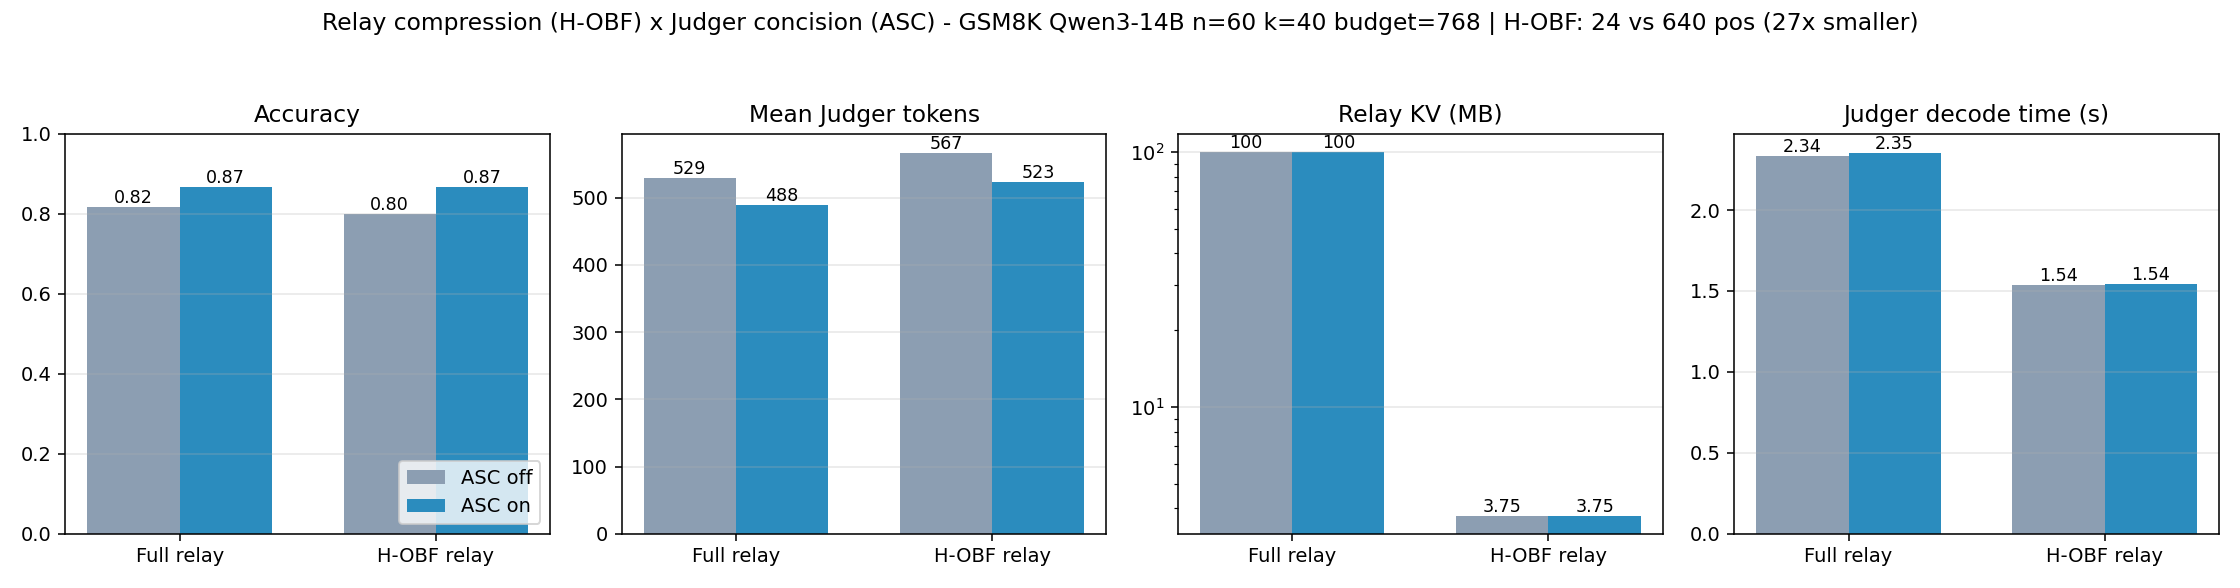
\includegraphics[width=\linewidth]{twobytwo_b16.png}
\caption{Aggressive compression ($\sim$27$\times$) on GSM8K. Near-iso accuracy;
verbosity tax removed by reader-side steering; faster decode on the small
cache. Full numbers in Table~\ref{tab:comp}.}
\label{fig:2x2}
\end{figure}

\paragraph{Whole-system accounting.}
Compression reduces relay memory and Judger decode cost; upstream latent
forwards to \emph{build} the cache remain. The honest win is memory and
throughput at the reader, not eliminating planning compute.
\todo{Stage-wise latency/memory Pareto across batch sizes.}

% ======================================================================
\section{Related Work}
\textbf{Latent multi-agent systems.} LatentMAS~\cite{latentmas} and text MAS
(debate, roles)~\cite{du2023debate} assume messages carry task content; we show
the \emph{latent} relay's benefit is largely content-independent and therefore
compressible.
\textbf{KV-cache compression.} H2O and SnapKV~\cite{h2o,snapkv} evict tokens in
single-context decoding; we show the same tools apply to a multi-agent latent
relay---and \emph{why} they are nearly free there.
\textbf{Activation steering.} CAA/SEAL~\cite{caa,seal} steer generation; we use
reader-side SEAL only as a verbosity control complementary to compression, and
show latent-channel steering does not raise accuracy.

% ======================================================================
\section{Discussion and Limitations}
\label{sec:limits}
\textbf{When compression is free.} Strongest on GSM8K with a capable 14B reader.
On MATH, instance-shuffle still holds but aggressive eviction costs accuracy:
compress gently, or accept a tax.

\textbf{AIME.} Prior K-sweep on this fork shows LatentMAS helps AIME at $K{=}10$
($0.67$ vs.\ $0.53$ at $K{=}0$). An exploratory AIME cache suite at $K{=}40$
collapsed absolute accuracy ($\sim$0.33) and is \emph{not} used for claims;
\todo{rerun AIME real/shuf/none/compress at $K{=}10$, budget 8192}.

\textbf{Other limits.} Single seed for several tables; MATH grading uses a light
normalizer; we do not claim upstream agents are useless---only that their benefit
is not carried by instance-specific latent content on the tasks tested.

\section{Conclusion}
The inter-agent KV cache in LatentMAS is not a problem-specific information
channel. That fact makes the relay compressible: \textbf{16--40$\times$} less
memory at matched accuracy on GSM8K, with reader-side steering handling
verbosity, and a harder-task boundary on MATH. Build latent multi-agent systems
assuming a redundant relay---compress it, and optimize the reader.

% ======================================================================
\begin{thebibliography}{9}
\small
\bibitem{latentmas} Zou et al. Latent Collaboration in Multi-Agent Systems.
arXiv:2511.20639, 2025.
\bibitem{seal} Chen et al. SEAL: Steerable Reasoning Calibration of LLMs for Free.
arXiv:2504.07986, 2025.
\bibitem{h2o} Zhang et al. H2O: Heavy-Hitter Oracle for Efficient Generative
Inference of LLMs. NeurIPS, 2023.
\bibitem{snapkv} Li et al. SnapKV: LLM Knows What You are Looking for Before
Generation. NeurIPS, 2024.
\bibitem{caa} Rimsky et al. Steering Llama 2 via Contrastive Activation Addition.
ACL, 2024.
\bibitem{du2023debate} Du et al. Improving Factuality and Reasoning in Language
Models through Multiagent Debate. ICML, 2024.
\end{thebibliography}

\end{document}
